\section{Background}
%\section{Modeling Data-Aware Declare Alignment}
%In this section, we introduce the requirements enabling the computation of data-aware declare alignments.

\subsection{Data-Aware Logs}
(Data) \textit{payloads} are finite functions $p\in V^K$, where $K$ is a finite set of keys and $V$ is a (finite) set of data values. We denote $\varPhi$ as an element $\varPhi\notin V$, such that $p(k)=\varPhi$ for $k\notin\textup{dom}(p)$. Given a finite set of activity labels $\textsf{Act}$, an event $\sigma_j$ is a pair $\Braket{\texttt{a},p}$, where $\texttt{a}\in\textsf{Act}$ is an activity label, and $p$ is a payload; we denote $\lambda$ (and $\varsigma$) as the first (and second) projection of such pair, i.e., $\lambda(\sigma_j)=\texttt{a}$ (and $\varsigma(\sigma_j)=p$). A \textit{trace} $\sigma$ is a temporally-ordered and finite sequence of distinct events $\sigma_1\cdots\sigma_n$, modeling a process run. We distinguish the trace keys ($K_t$) from the event keys ($K_e$), such that $K=K_t\cup K_e$ with $K_t\cap K_e=\emptyset$: all events within the same trace associate the same values to the same trace keys, i.e., $\forall \Braket{\texttt{a}_i,p_i},\Braket{\texttt{a}_j,p_j}\in\sigma.\;\forall k\in K_t.\; p_i(k)=p_j(k)$. A log $\mathcal{L}$ is a finite set of traces. This  characterization is compliant with the \textsc{eXtensible Event Stream} format, which is the \textit{de facto} standard for representing event logs within the Business Process Management community \cite{SchonigCMM16,LenoDM18}.


\subsection{Data-Aware Declare}\label{ssec:dad}
\textsc{Declare} is a constraint-based process modeling language, where a Declare model $\mathcal{M}$ is described as a set of constraints $\Set{c_1,\dots,c_m}$ that must be simultaneously satisfied throughout the process execution. Due to space limitations, we avoid providing a detailed description of Data-Aware Declare \cite{SchonigCMM16,LenoDM18}, henceforth simply referred as Declare, and we will only describe its general features.

 Such constraints express either positive (or negative) dependencies between two events having labels in $\textsf{Act}$, or quantify the occurrence of events having a specific label in $\textsf{Act}$. In the first case, one of the two clause labels is called \textit{activation}, and the other \textit{target}; while testing a trace $\sigma$ for conformance over such clause, the presence of the activation label in $\sigma$ triggers the clause verification, requiring the execution of an event containing the target label in the same trace. The conditions over the activation (or target) labels \texttt{a} can be expressed via predicates $\phi_{\texttt{a}}$ \cite{SchonigCMM16,LenoDM18}. Activations and targets can be additionally decorated with  data predicates $\phi^d$ (\textit{conditions}): while activation conditions must be valid when the activation label occurs within the event exhibiting such label, target conditions impose value limitations on events containing such target label. We denote the \textit{compound conditions}, namely the conjunction of label requirements and data conditions, as $\psi=\phi_{\texttt{a}}\wedge \phi^d$.  Even if current literature  considers \textit{correlation} conditions between activations and targets \cite{SchonigCMM16}, we will not model such constraints as previously discussed in \S\ref{sec:mot}. Such constraints can be represented by either an intuitive graphical representation, which makes them easy to use and interpret for process analysts, or with a formal semantics \cite{LeoniMA12}.

\begin{figure}[!t]
	\centering
%	\begin{subfigure}[b]{0.45\textwidth}
%		\centering
%		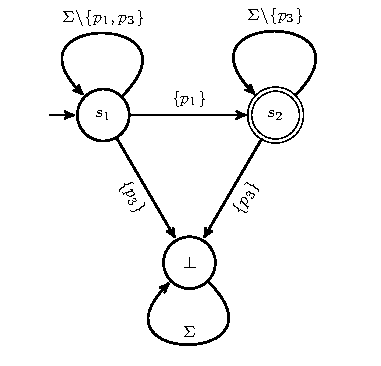
\includegraphics[width=\textwidth]{images/example_1_graph}
%		\caption{$\bot\Release(\neg p_3\vee p_1\vee p_2) \wedge \top\mathcal{U}p_1$}
%		\label{fig:g1}
%	\end{subfigure}
%	\hfill
%	\begin{subfigure}[b]{0.45\textwidth}
%
%	\end{subfigure}
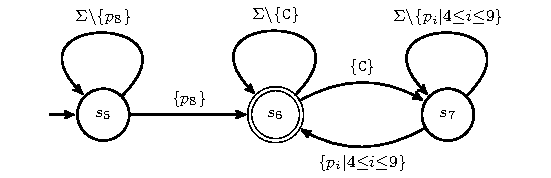
\includegraphics[scale=0.9]{images/example_3_graph}
%\caption{$\bot\Release(\neg\texttt{A}\vee(\top\Until(p_2\vee p_3)))\wedge\top\Until p_3$}
%\label{fig:g2}
	\caption{Representation of an LTL$_f$ formula $\bot\mathcal{R}(\neg\texttt{A}\vee(\top\mathcal{U}(p_4\vee p_5\vee p_6\vee p_7\vee p_8\vee p_9)))\wedge\top\mathcal{U} p_8$  as a constraint automaton from \cite{LeoniMA12,Westergaard11}, where $\Sigma$ contains all the non-$\bot$ and non-$\top$ atoms.}
	\label{fig:g1g2}
\end{figure}

\subsection{Working Assumptions}\label{sec:wa}
In this section, we outline some working assumptions that can be inferred from the literature of reference. First, we assume that we only want to align declare models over  log traces \cite{XuLZ17a}; this implies that \begin{enumerate*}[label=\emph{\alph*})] \item compliance requirements of Declare models can be expressed in a formal language such as Linear Time Logic on Finite Traces (LTL$_f$) \cite{10.1007/978-3-642-40176-3_8}, as logs are finite sets of finite traces \cite{GiacomoV13}; \item differently from \cite{BurattinMS16,MaggiMB19}, we work under the closed world assumption, as the only possible set of traces that might satisfy a Declare constraints might come from its associated constraint automaton and, possibly, from the set of log traces; \item differently from \cite{MultiPerspective}, we can avoid to model reading and writing operation, as the entirety of our analyses will be conducted \textit{post-mortem}; \item last, each event trace must be represented by one single proposition \cite{XuLZ17a}. \end{enumerate*} As we will see in the incoming section, the latter consideration will require us to partition the possible data space into distinct propositions. 




%Still, we can freely assume that the constraint automatons generated from the LTL$_f$ interpretation of such Declare constraints allow to represent any possible event label that is not represented within the Declare constraints, by either representing it as a transition $\Sigma\backslash S$, where $\Sigma$ is the set of all the possible strings and $S$ is a (possibly empty) finite set of traces that we want to ignore \cite{LeoniMA12,Westergaard11}, or by representing it as finite conjunction of negated predicates \cite{Lydia}, where each predicate is a proposition that can be deduced from a Declare Model represented in LTL$_f$. Figure~\ref{fig:g1g2} provides a intuitive representation of some LTL$_f$ formulae in the former representation.

We can freely assume that %%activation and target with data conditions can be expressed as a propositional formula $\psi(\sigma_i):=\phi_{\texttt{a}}(\sigma_i)\wedge \phi^d(\sigma_i)$ for each event $\sigma_i$ \cite{LenoDM18}, where $\phi_{\texttt{a}}(\sigma_i)$ denotes a predicate $\lambda(\sigma_i)=\texttt{a}$ over the activation (or target) label \texttt{a}, $\phi^d(\sigma_i)$ denotes the associated data condition over $\varsigma(\sigma_i)$. 
$\phi_\texttt{a}$ for $\texttt{a}\in\textsf{Act}$ can be expressed as an atom $\lambda(\sigma_i)=\texttt{a}$ for a given event $\sigma_i$ to be assessed, while $\phi^d$ is a propositional formula containing as atoms either
%%The latter is a
%Firstly, $\phi_{\texttt{a}}(\sigma_i)$ is always an atomic predicate $\lambda(\sigma_i)=\texttt{a}$ over the activation (or target) label $\texttt{a}\in\textsf{Act}$; such predicates are usually denoted simply as ``\texttt{a}'' \cite{XuLZ17a}. Secondly, $\phi^d(\sigma_i)$ is yet another
%%propositional formula containing either 
the universal truth ($\top$), or the falsehood ($\bot$), or a %%predicate in the form ``$\varsigma(\sigma_i)(k)\;\Re\;c$'', usually denoted as ``$\texttt{a}.k\;\Re\;c$''; such predicate puts in relation $\Re$ the value associated to the key $k\in K$ within  payload $\varsigma(\sigma_i)$ to a constant value $c$, %where the data value $\varsigma(\sigma_i)(k)$ associated to the key $k$ within the payload $\varsigma(\sigma_i)$ o 
binary relation ``$\texttt{a}.k\;\Re\;c$'', where $c$ is a constant value 
%
%
%, as well as their associated conditions, can be expressed in propositional logic over one single event $\sigma_i$. With respect to the activity label conditions for events $\sigma_i$, we can express those as a single atomic predicate in the form ``$\lambda(\sigma_i)=\texttt{a}$'' for each $\texttt{a}\in\textsf{Act}$; we will use ``\texttt{a}'' as a shorthand for such predicates. With respect to the (data) conditions, we assume that each atomic predicate refers to 
%
%We assume that the conditions for Declare clauses are always expressed in propositional calculus, where the atomic predicates are always in the form ``$\texttt{A}.\textit{var}\;\Re\; c$'', where \texttt{A} is a trace label containing a property named \textit{var} which is put in a binary relation $\Re$ with a constant value $c$, 
representing either a number or a string, $\Re$ is either an equality or a precedence/subsequent relation over values in $V$ or their negation, and $k\in K$ acts as a placeholder for $\varsigma(\sigma_i)(k)$, where $\varsigma(\sigma_i)$ is the payload associated to the event $\sigma_i$ and $k$ is associated to a value $\sigma(\sigma_i)(k)$. E.g., ``$\texttt{RP}.\textit{quality}\leq 3$'' is formally represented as $\varsigma(\sigma_i)(k)\leq 3$ for any event $\sigma_i$ having $\lambda(\sigma_i)=\texttt{RP}$.  This is a widely adopted assumption, that spans from data-aware procedural models \cite{MultiPerspective} to data-aware declarative models \cite{10.1007/978-3-642-40176-3_8}. Furthermore, this assumption can be also adapted to categorical data, as strings are ordered via lexicographical orderings over the single characters \cite{MultiPerspective}.

Given an appropriately choosen set $\Sigma$ of atoms, it is always possible to represent a trace $\sigma=\sigma_1\cdots \sigma_n$ as a finite sequence $t_\sigma=t_1\cdots t_n$, where it always exists an unique atom $t_i\in\Sigma$ such that $\sigma_i\vDash t_i$ for $1\leq i\leq n$ \cite{XuLZ17a,MaggiMCA18}. 
Contextually,  any LTL$_f$ $\varphi_{\mathcal{M}}$ representing a Declare model $\mathcal{M}$ can be represented as a deterministic finite-state automaton (DFA) $\mathcal{A}_{\varphi_{\tiny\mathcal{M}}}$ \cite{Westergaard11,Lydia} accepting all the sequences $t_\sigma$ from traces $\sigma$ satisfying $\varphi$ (Figure~\ref{fig:g1g2}). A DFA  $(\Sigma,Q,q_0,\rho,F)$ is defined \cite{0016921} over a finite set of states $Q$ reading as an input symbols from a finite alphabet $\Sigma$ that are consumed by traversing the automaton from a starting state $q_0\in Q$ via a transition function $\rho\colon Q\times \Sigma\to Q$; the input sequence is accepted once the input sequence is completely digested and an accepting state in $F\subseteq Q$ is reached through navigation. Given that in the non data-aware scenario the atoms within LTL$_f$ could be either $\top$, or $\bot$, or $\psi=\phi_\texttt{a}$ for $\texttt{a}\in\textsf{Act}$, $\Sigma$ corresponds to the set of label requirements $\Set{\phi_\texttt{a}|\texttt{a}\in\textsf{Act}}\sim\textsf{Act}$, as each event is associated to one single label.

Last, we freely assume that all the events having the same label will always contain the same set of keys, with possibly differently associated values. This is a common assumption in relational database field, where all the rows belonging to the same table contain the same number of values. We also freely assume that missing values are represented with specific values, such as an empty string, $-1$, $0$, $-\infty$, or $+\infty$, depending on the context.